\chapter{华为云DevCloud}

本次课程作业在华为云DevCloud上完成,华为云在上面一站式提供了项目规划、代码管理、
持续集成、持续部署、文档编写等功能,涉及项目开发的几乎所有方面。
本文对其持续集成和持续部署方面进行介绍和总结。

在华为云的构建\&发布中,共涉及流水线、编译构建、部署、发布和运维五部分。
本次课程作业中主要涉及了前三部分,发布和运维暂无涉及。

\begin{figure}[h]
    \centering
    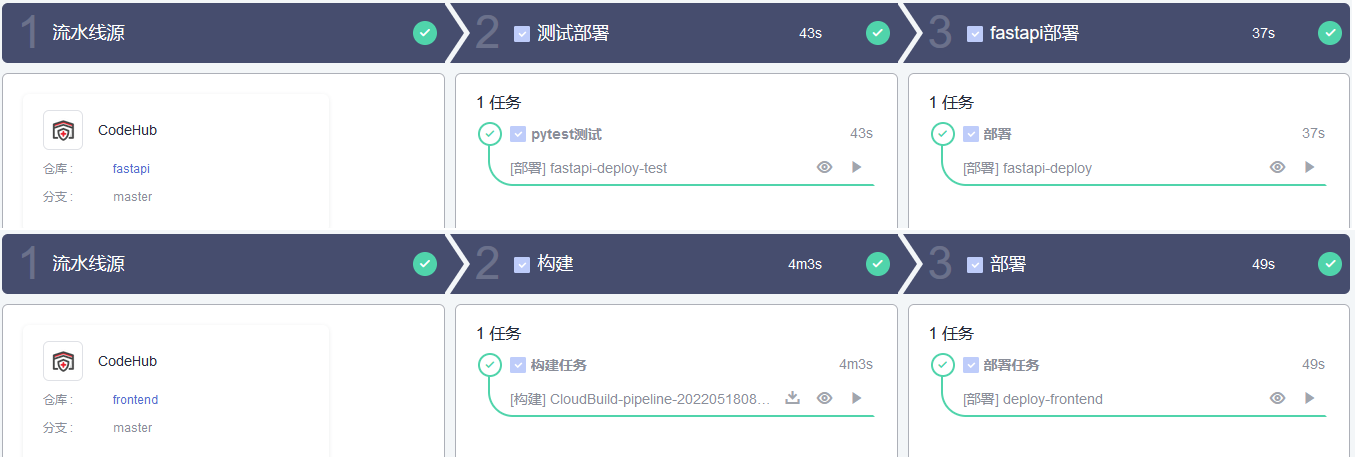
\includegraphics[width=1\textwidth]{figures/huawei/pipeline.png}
    \caption{华为云流水线}
    \label{fig:huawei_pipeline}
\end{figure}

在图\ref{fig:huawei_pipeline}中,展示了两条前端流水线。流水线会绑定一个代码仓库,
当满足触发条件后按顺序执行流水线上的操作。操作有多种,
本例中前端的流水线为构建镜像并部署,后端的流水线为先进行测试部署再进行部署。
当前阶段出现错误后,流水线默认会自动停止执行。
以后端为例,如果某次代码变动导致代码未通过测试部署,那么将会停止流水线,
从而避免错误代码直接部署上线。

\begin{figure}[h]
    \centering
    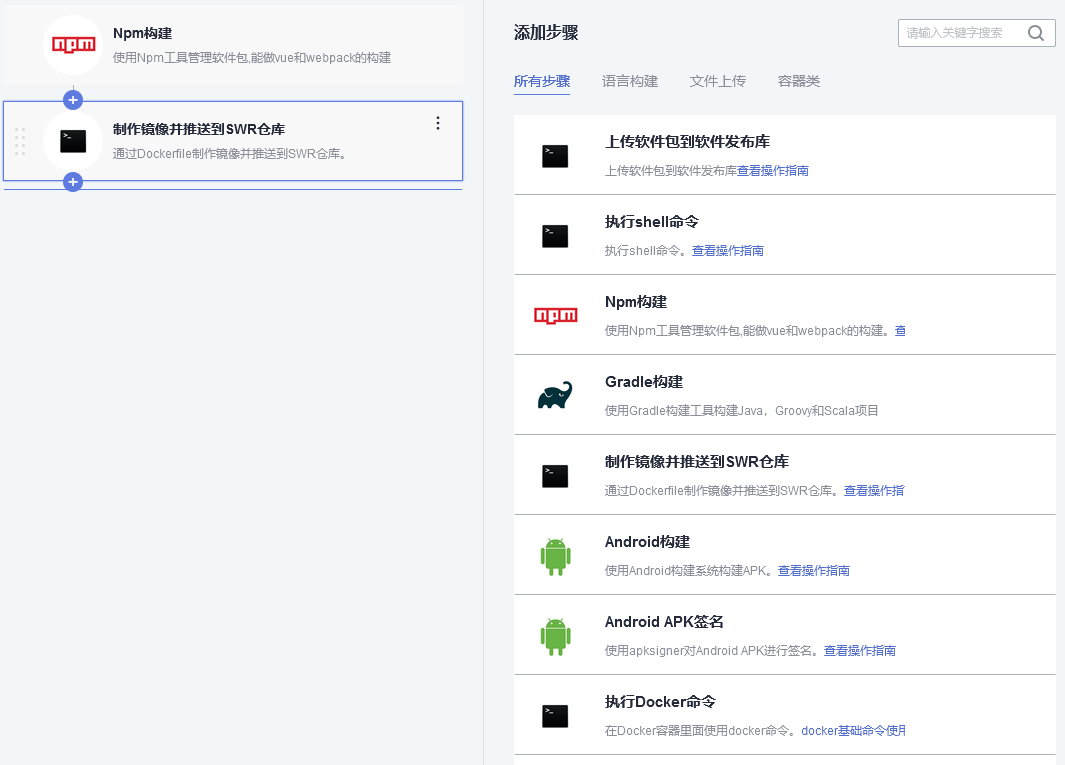
\includegraphics[width=1\textwidth]{figures/huawei/build.png}
    \caption{华为云编译和构建}
    \label{fig:huawei_build}
\end{figure}

流水线每个阶段执行的任务在编译构建和部署中事先创建,并在流水线中被引用。
相比AppVeyor和GitHub Actions中需要自己编写配置文件,图\ref{fig:huawei_build}中看到
华为云以可视化的方式提供了丰富的步骤, 让开发人员不用手动编写构建或者部署代码。

相比其他重点在持续集成的平台,由于华为云自己就提供云主机的服务,
因此提供了主机组管理的功能。华为云支持将多台主机指定为一个主机组,
部署时可以针对整个主机组一次性全部部署,降低了部署工作量。